% 2010 年辽宁卷文科第 16 题：网格纸上的三视图（正视图、侧视图、俯视图）。
% 来源 PDF：普通高考/2010/2010辽宁文.pdf，SHA-256 b402a859318cb9854e9b8257ea128e84f1d52e834556dd80625e883f88dea1fd。
% 原页：第 1 页（A3 三栏）第 2 栏下部，书页码 613。
% 重绘依据：照原页 L 形网格（8 列 × 8 行，左下块占 x=0..4、y=0..4，上部满宽 8 列 × 4 行）：
%   左上是正视图（直角边 2、2，直角在右下，斜边自左下至右上），
%   右上是侧视图（直角边 2、2，直角在左下，斜边自左上至右下），
%   左下是俯视图（边长 2 的正方形加一条自左下至右上的对角线）。
%   网格用细灰线，三视图轮廓用粗黑线。
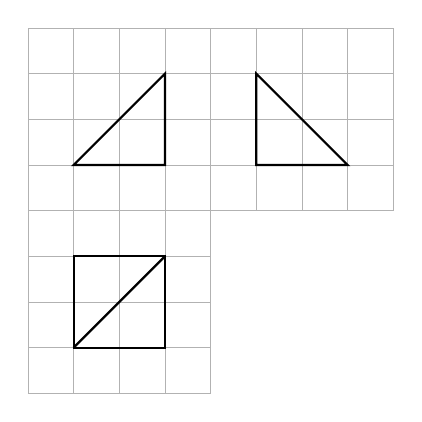
\begin{tikzpicture}[scale=0.58]
  % 横线：上半满宽（x=0..8），下半仅左四列（x=0..4）
  \foreach \y in {0,1,2,3} {
    \draw[gray!60, very thin] (0,\y) -- (4,\y);
  }
  \foreach \y in {4,5,6,7,8} {
    \draw[gray!60, very thin] (0,\y) -- (8,\y);
  }
  % 竖线：左四列满高，右上四列只在上半
  \foreach \x in {0,1,2,3,4} {
    \draw[gray!60, very thin] (\x,0) -- (\x,8);
  }
  \foreach \x in {5,6,7,8} {
    \draw[gray!60, very thin] (\x,4) -- (\x,8);
  }

  % 正视图（左上）：直角边 2、2，斜边自左下至右上
  \draw[thick] (1,5) -- (3,5) -- (3,7) -- cycle;
  % 侧视图（右上）：直角边 2、2，斜边自左上至右下
  \draw[thick] (5,5) -- (7,5) -- (5,7) -- cycle;
  % 俯视图（左下）：边长 2 的正方形加一条对角线
  \draw[thick] (1,1) rectangle (3,3);
  \draw[thick] (1,1) -- (3,3);
\end{tikzpicture}
